%%%%%%%%%%%%%%%%%%%%%%%%%%%%%%%%%%%%%%%%%%%%%%%%%%%%%%%%%%%%%%%%%%%%%%%%%%%%%
%
%  System        : 
%  Module        : 
%  Object Name   : $RCSfile$
%  Revision      : $Revision$
%  Date          : $Date$
%  Author        : $Author$
%  Created By    : Robert Heller
%  Created       : Mon Aug 29 11:04:14 2022
%  Last Modified : <221115.1606>
%
%  Description 
%
%  Notes
%
%  History
% 
%%%%%%%%%%%%%%%%%%%%%%%%%%%%%%%%%%%%%%%%%%%%%%%%%%%%%%%%%%%%%%%%%%%%%%%%%%%%%
%
%    Copyright (C) 2022  Robert Heller D/B/A Deepwoods Software
%			51 Locke Hill Road
%			Wendell, MA 01379-9728
%
%    This program is free software; you can redistribute it and/or modify
%    it under the terms of the GNU General Public License as published by
%    the Free Software Foundation; either version 2 of the License, or
%    (at your option) any later version.
%
%    This program is distributed in the hope that it will be useful,
%    but WITHOUT ANY WARRANTY; without even the implied warranty of
%    MERCHANTABILITY or FITNESS FOR A PARTICULAR PURPOSE.  See the
%    GNU General Public License for more details.
%
%    You should have received a copy of the GNU General Public License
%    along with this program; if not, write to the Free Software
%    Foundation, Inc., 675 Mass Ave, Cambridge, MA 02139, USA.
%
% 
%
%%%%%%%%%%%%%%%%%%%%%%%%%%%%%%%%%%%%%%%%%%%%%%%%%%%%%%%%%%%%%%%%%%%%%%%%%%%%%

\chapter{ESP32-S3-MultiFunction: Multifunction board using an ESP32-S3FN8}

This is a LCC\footnote{Layout Command Control, See
\url{https://www.nmra.org/lcc} for more details and available standards
documentation.} node circuit board that is based around an Espressif
ESP32-S3FN8 MCU to manage and operate a collection of model railroad sensors
and actuators. The board contains these I/O sections:

\begin{itemize}
\item Four occupancy detectors. CT Coil type sensors, so they won't work with
DC systems without an AC bias. 
\item Four stall-motor drivers with point sense. 
\item Four Schmitt Trigger inputs, meant for push buttons. 
\item Four Buffered outputs, by default for Panel LEDS, but with drop in
resistors, can also drive relays or other loads. 
\item Sixteen PWM Led drivers. These are meant to light (LED) lamps in signal
heads.
\end{itemize}

The board connects to a LCC network and utilizes the Event Transport Protocol
in its operation. It also uses a CDI\footnote{Configuration Description
Information.} to describe its configuration. It can be configured with JMRI or
other available LCC configuration tools.

The board draws about 30ma, plus load. Circuitron specifies that a Tortoise
switch machine draws about 16ma when stalled, so four Tortoise switch machines
would add 64ma. There is a terminal block near the stall motor terminal blocks
to optionally provide external power for the switch machines. There are 16
signal lamp outputs that have 1.5K Ohm load resistors, this means about 8ma
per LED. If all lamps are on at full briteness, this comes to 128ma, although
turning all 16 signal on full at a time is not likely to be prototypical,
since most signal aspects only light one lamp per head. There is a terminal
block to optionally supply external power for the signal lamps, as a way to
reduce the load on the LCC power bus. The buffered output section uses an
external power source, so does not add any load to the LCC power bus.

This board is a multi-purpose board that can be used in a number of 
situations, including (but not limited to): one end of a siding, a yard or 
terminal throat, ABS, and interlocking plants.

\clearpage
\section{Circuit Description}

\subsection{Section Interconnect}
\begin{figure}[hbpt]\begin{centering}%
\includegraphics[width=4in]{ESP32-S3-MultiFunction-1.pdf}
\caption{Circuit Diagram of the ESP32-S3-MultiFunction board, page 1: Main 
sheet -- Section Interconnect}
\end{centering}\end{figure}
\begin{figure}[hbpt]\begin{centering}%
\includegraphics{ESP32-S3-MultiFunction-top3D.png}
\caption{3D Rendering of the whole board.}
\end{centering}\end{figure}

This shows how the various subsections are interconnected.
\clearpage
\subsection{MCU}
\begin{figure}[hbpt]\begin{centering}%
\includegraphics[width=4in]{ESP32-S3-MultiFunction-2.pdf}
\caption{Circuit Diagram of the ESP32-S3-MultiFunction board, page 2: MCU}
\end{centering}\end{figure}
\begin{figure}[hbpt]\begin{centering}%
\includegraphics{ESP32-S3-MultiFunction-top3D-MCU.png}
\caption{3D Rendering of the MCU section.}
\end{centering}\end{figure}

This is the MCU and its closely related circuitry, including bypass caps, USB 
connection (for programming and debugging), reset and boot buttons and 
activity LEDS.  There is a micro-B USB connector for programming and 
debugging. 

%\clearpage
\subsection{3.3V Power Supply}
\begin{figure}[hbpt]\begin{centering}%
\includegraphics[width=4in]{ESP32-S3-MultiFunction-3.pdf}
\caption{Circuit Diagram of the ESP32-S3-MultiFunction board, page 3: 3.3V 
Power Supply}
\end{centering}\end{figure}
\begin{figure}[hbpt]\begin{centering}%
\includegraphics{ESP32-S3-MultiFunction-top3D-PowerSupply.png}
\caption{3D Rendering of the 3.3V Power Supply section.}
\end{centering}\end{figure}

This is the 3.3 volt power supply for all of the logic circuits.

%\clearpage
\subsection{LED Drivers and Buttons}
\begin{figure}[hbpt]\begin{centering}%
\includegraphics[width=3.5in]{ESP32-S3-MultiFunction-4.pdf}
\caption{Circuit Diagram of the ESP32-S3-MultiFunction board, page 4: LED 
Drivers and Button Inputs}
\end{centering}\end{figure}
\begin{figure}[hbpt]\begin{centering}%
\begin{minipage}{.45\textwidth}
  \centering
  \includegraphics{ESP32-S3-MultiFunction-top3D-LEDDrivers.png}
  \caption{3D Rendering of the LED Drivers Section.}
  \label{fig:ESP32-S3-MultiFunction-top3D-LEDDrivers}
\end{minipage}
\begin{minipage}{.45\textwidth}
  \centering
  \includegraphics{ESP32-S3-MultiFunction-top3D-Buttons.png}
  \caption{3D Rendering of the Buttons Section.}
  \label{fig:ESP32-S3-MultiFunction-top3D-Buttons}
\end{minipage}\end{centering}\end{figure}

This is the driver ciruits for the generic LED (or other devices) outputs and
the four push button inputs. The driver outputs have 1.5K Ohm resistors
soldered to the board, which limits the current to about 10ma at 12V and have
places to solder through hole resistors to bypass these resistors to allow for
higher currents (up to 1.5A). The outputs need an external (nomially 12V,
referenced to system ground) supply for these outputs.

The four inputs are buffered with Schmitt Triggers, which provides hardware 
bounce processing.

There is a 6 position (2.54mm pitch) screw terminal for the LED Driver 
outputs.  One end is for the +V (nomially 12V) power source and the other end 
is the ground (-) connection.  In between these terminals are the four 
outputs, which can be driven either high or low.

For the button inputs there is a 5 position (2.54mm pitch) screw terminal 
block. One end is common ground and the other four are for the four buttons.

\subsection{Turnout Control} 
\begin{figure}[hbpt]\begin{centering}%
\includegraphics[width=4in]{ESP32-S3-MultiFunction-5.pdf}
\caption{Circuit Diagram of the ESP32-S3-MultiFunction board, page 5: Turnout 
Drivers and Point Sense}
\end{centering}\end{figure}
\begin{figure}[hbpt]\begin{centering}%
\includegraphics{ESP32-S3-MultiFunction-top3D-Turnouts.png}
\caption{3D Rendering of the Turnouts Section.}
\end{centering}\end{figure}

The Turnout Control section has two parts, a driver part and a sense part.  
For each turnout there is a 5 position (2.54mm pitch) screw terminal block, 
with the connections MA, MB, PA, GND PB.   The MA and MB drive the motor at 
nominally 12 volts.  The PA and PB with the GND connection expect a SPST 
switch mechanically connected to the points (one pole of the internal switch 
in a Tortoise switch motor will work as well).

\clearpage
\subsection{Occupancy Detectors}
\begin{figure}[hbpt]\begin{centering}%
\includegraphics[width=4in]{ESP32-S3-MultiFunction-6.pdf}
\caption{Circuit Diagram of the ESP32-S3-MultiFunction board, page 6: 
Occupancy Detectors}
\end{centering}\end{figure}
\begin{figure}[hbpt]\begin{centering}%
\includegraphics{ESP32-S3-MultiFunction-top3D-OccupancyDetectors.png}
\caption{3D Rendering of the Occupancy Detectors Section.}
\end{centering}\end{figure}

The occupancy detector circuits use a pair of comparitors to detect current in 
a current transformer coil (CT Coil) that would have a track power feeder 
going through it.  The sensitivity can be adjusted and there are indicator 
LEDS on the board.  There is an 8 position (2.54mm pitch) screw terminal 
block, adjacent pairs of terminals are used for each detector.

%\clearpage
\subsection{PWM Signal Lamp drivers}
\begin{figure}[hbpt]\begin{centering}%
\includegraphics[width=4in]{ESP32-S3-MultiFunction-7.pdf}
\caption{Circuit Diagram of the ESP32-S3-MultiFunction board, page 7: PWM 
Signal Lamp drivers}
\end{centering}\end{figure}
\begin{figure}[hbpt]\begin{centering}%
\includegraphics{ESP32-S3-MultiFunction-top3D-PWMSignalLamps.png}
\caption{3D Rendering of the PWM Signal Lamps Section.}
\end{centering}\end{figure}

The PWM Signal Lamp drivers use a PCA9685 which is a 16 channel, 12 bit PWM
LED driver. A pair of octal MOSFET drivers and series load resistors are also
included on the board. The MOSFET drivers come in both inverting (low-side
drive) and non-inverting (high-side drive), so it is possible to support both
common anode and common cathode LED signals. 

There are two 9 position (2.54mm pitch) screw terminal blocks, one for each
bank of 8 lamps (A and B), with a common terminal for each. There is also a 2
position (2.54mm pitch) screw terminal block to optionally provide separate
power for the Signal Lamps.

%\clearpage
\subsection{CAN Transceiver}
\begin{figure}[hbpt]\begin{centering}%
\includegraphics[width=4in]{ESP32-S3-MultiFunction-8.pdf}
\caption{Circuit Diagram of the ESP32-S3-MultiFunction board, page 8: CAN 
Transceiver}
\end{centering}\end{figure}
\begin{figure}[hbpt]\begin{centering}%
\includegraphics{ESP32-S3-MultiFunction-top3D-CANTransceiver.png}
\caption{3D Rendering of the CAN Transceiver  Section.}
\end{centering}\end{figure}

The CAN Transceiver (TCAN332DR) converts the TTL CAN TX and CAN RX signals to 
CAN\_H and CAN\_L signals and connects them to the pair a parallel wired RJ45 
jacks.  There is also a termination jumper block and 2 position (2.54mm pitch) 
screw terminal blocks to access power in or out of the CAN network.

\clearpage

\section{General Wiring Notes}

There are various terminal blocks, connectors, and jumper blocks on this 
board.  At the bottom edge near the center of the board are a pair of two 
position terminal blocks, one for injecting power into the LCC bus and one for 
extracting power from the LCC bus. Between these terminal blocks is the 
termination jumper block for the LCC bus.  Above the LCC power terminal blocks 
is a pair of RJ45 connectors. These are for connecting the board to the LCC 
bus. These connectors are wired in parallel. Down along the left side 
are the four stall motor terminal blocks (5 position terminal blocks) 
and the occupancy detector terminal block (8 position terminal block).  On the 
lower left edge of the board is a 6 position terminal block for the LED Driver 
outputs and on the lower right edge is a 5 position terminal block for the 
input buttons.  On the right side are two 9 position terminal blocks for the 
signal lamp LEDs. Finally, between the terminal blocks for the signal lamp 
LEDs is a two position terminal block to (optionally) provide power for the 
signal lamp LEDs.

\subsection{LCC Power}

Power can be optionally injected into the LCC bus or extracted from the LCC 
bus. Power can be injected to into the LCC bus to power this and other boards. 
Power can also be extracted to power local devices.

\subsection{LCC Bus connections and termination}

\begin{figure}[hbpt]\begin{centering}%
\includegraphics{ESP32-S3-MultiFunction-termination.png}
\caption{Termination Jumper Options}
\label{fig:ESP32-S3-MultiFunction-termination}
\end{centering}\end{figure}
The two RJ45 connections connect to the LCC bus.  If this board is at the end 
of bus, you will need to terminate the bus.  There are two possible 
termination options as shown in 
Figure~\ref{fig:ESP32-S3-MultiFunction-termination}.  With no jumpers 
installed the bus is not terminated, with jumpers installed horizontally 
(parallel to the bottom edge), you will have simple termination (120 Ohms 
across the CAN bus), with jumpers installed vertically, you will have 
center-tap termination (with a 47pf cap to ground).

\subsection{Stall Motors connections}
\label{sec:StallMotorsconnections}
\begin{figure}[hbpt]\begin{centering}%
\includegraphics{ESP32-S3-MultiFunctionTurnoutMotorsFig.png}
\caption{Stall Motor terminal block connections}
\label{fig:ESP32-S3-MultiFunctionTurnoutMotorsFig}
\end{centering}\end{figure}
\begin{figure}[hbpt]\begin{centering}%
\includegraphics[height=2in]{ESP32-S3-MultiFunctionTotoiseWiring.png}
\caption{Wiring a Tortoise to the ESP32-S3-MultiFunction Turnout Motors terminals}
\label{fig:ESP32-S3-MultiFunctionTotoiseWiring}
\end{centering}\end{figure}

The five position Stall Motor terminal blocks, shown in 
Figure~\ref{fig:ESP32-S3-MultiFunctionTurnoutMotorsFig}, connect to the 
turnout stall motors, the Motor A and Motor B connections go to the motor 
(pins 1 and 8 of a tortoise), the other three connections go to a single pole 
double throw switch contacts to sense the position of the stall motor / 
points. There are contacts available on tortoise stall motor that can be used 
for this purpose, as shown in 
Figure~\ref{fig:ESP32-S3-MultiFunctionTotoiseWiring}\footnote{Depending on how 
the motor is positioned and the ``sense'' of the position, the A/B connections 
can be swapped to suit.}.

There is a two position terminal block to optionally provide power for the
stall motors.

\subsection{Occupancy Detector connections}
\begin{figure}[hbpt]\begin{centering}%
\includegraphics{ESP32-S3-MultiFunctionOccupancyDetectorsTermBlock.png}
\caption{Occupancy Detectors Terminal Block}
\label{fig:ESP32-S3-MultiFunctionOccupancyDetectorsTermBlock}
\end{centering}\end{figure} 
\begin{figure}[hbpt]\begin{centering}%
\includegraphics[height=1.5in]{ESP32-S3-MultiFunctionOccupancyDetectorsCTCoilWiring.png}
\label{fig:ESP32-S3-MultiFunctionOccupancyDetectorsCTCoilWiring}
\caption{Wiring a CT Coil to the Occupancy Detectors Terminal Block}
\end{centering}\end{figure}

The eight position Occupancy Detector terminal block, shown in 
Figure~\ref{fig:ESP32-S3-MultiFunctionOccupancyDetectorsTermBlock}, connect to 
the CT Coils, as shown in 
Figure~\ref{fig:ESP32-S3-MultiFunctionOccupancyDetectorsCTCoilWiring}.  Using 
twisted pair wires is recogmended.  A good source of twisted pairs is Ethernet 
cable (Cat5).



\subsection{Signal Lamp (LED) connections}
\begin{figure}[hbpt]\begin{centering}%
\includegraphics{ESP32-S3-MultiFunction-PWMSignalLampTerminalBlocks.png}
\caption{PWM Signal Lamp Terminal Block}
\label{fig:ESP32-S3-MultiFunction-PWMSignalLampTerminalBlocks}
\end{centering}\end{figure}
\begin{figure}[hbpt]\begin{centering}%
\includegraphics{ESP32-S3-MultiFunction-PWMSignalLampWiring.png}
\caption{Typical Signal Lamp Diver Wiring}
\label{fig:ESP32-S3-MultiFunction-PWMSignalLampWiring}
\end{centering}\end{figure}

There are two Signal lamp terminal blocks, as shown in 
Figure~\ref{fig:ESP32-S3-MultiFunction-PWMSignalLampTerminalBlocks}. Each 
terminal block has eight terminals for signal lamp LEDs, plus a common.  A 
typical signal head would be wired as shown in 
Figure~\ref{fig:ESP32-S3-MultiFunction-PWMSignalLampWiring}.

\subsection{LED/Driver outputs}
\begin{figure}[hbpt]\begin{centering}%
\includegraphics{ESP32-S3-MultiFunctionLEDDriverWiring.png}
\caption{Wiring the LED Driver outputs.}
\label{fig:ESP32-S3-MultiFunctionLEDDriverWiring}
\end{centering}\end{figure}

The LED / Driver outputs, shown in 
Figure~\ref{fig:ESP32-S3-MultiFunction-top3D-LEDDrivers}, can be used to drive 
standard LEDs and can also be used to drive heavier loads, by adding resistors 
to bypass the on board 1.5K Ohm resistors, as shown in 
Figure~\ref{fig:ESP32-S3-MultiFunctionLEDDriverWiring}.

The LED / Driver outputs require an external DC power source, typically 12V,
but it can be between 4.5VDC to 18VDC. These outputs are push/pull, so they
can drive either high-side or low-side loads, upto 1.5A.

\subsection{Push Button inputs}
\begin{figure}[hbpt]\begin{centering}%
\includegraphics{ESP32-S3-MultiFunction-ButtonsTerminalBlock.png}
\caption{Button input terminal block}
\label{fig:ESP32-S3-MultiFunction-ButtonsTerminalBlock}
\end{centering}\end{figure}
\begin{figure}[hbpt]\begin{centering}%
\includegraphics{ESP32-S3-MultiFunctionButtonWiring.png}
\caption{Wiring a button}
\label{fig:ESP32-S3-MultiFunctionButtonWiring}
\end{centering}\end{figure}

The buttons terminal block, shown in 
Figure~\ref{fig:ESP32-S3-MultiFunction-ButtonsTerminalBlock}, allows for 4 
push buttons switches, which would be wired as shown in 
Figure~\ref{fig:ESP32-S3-MultiFunctionButtonWiring}.

\clearpage
\section{Configuration}

\subsection{Occupancy Detectors}

Each occupancy detector entry has these configuration settings:

\begin{enumerate}
\item \textbf{Description} This is a user description of the block. 15 
characters.  Typically this is the name of the block.
\item \textbf{Debounce parameter} Amount of time to wait for the input to 
stabilize before producing the event. Unit is 30 msec of time. Usually a value 
of 2-3 works well in a non-noisy environment. In high noise (train wheels for 
example) a setting between 8 -- 15 makes for a slower response time but a more 
stable signal.

Formally, the parameter tells how many times of tries, each 30 msec apart, the 
input must have the same value in order for that value to be accepted and the 
event transition produced.
\item \textbf{Block Occupied} This event will be produced when the block 
becomes occupied.
\item \textbf{Block Clear} This event will be produced when the block becomes 
clear.
\end{enumerate}

The debounce parameter can be adjusted depending on how ``noisy'' the signal 
is.  Otherwise the configuration is just the name of the block and the two 
produced events.

\subsection{Turnouts}

Each turnout entry has these configuration settings:

\begin{enumerate}
\item \textbf{Description} This is a user description of the turnout. 8 
characters.  Typically this is the name of the turnout.
\item \textbf{Normal} Receiving this event ID will align the turnout to 
normal.
\item \textbf{Reversed} Receiving this event ID will align the turnout to 
reversed.
\item \textbf{Veto On} Receiving this event ID will lock the turnout.
\item \textbf{Veto Off} Receiving this event ID will unlock the turnout.
\end{enumerate}

The configuration is just the name and the four consumed events. The default
veto state is ``off'', so the Veto On and Veto Off events can be just not
used, but they are available to lock and unlock the turnout, should that be
desirable.  Typically, the OS section occupancy detector events can be used 
here to lock the turnout when a train is occupying the turnout.

\subsection{Points}

Each points entry has these configuration settings:

\begin{enumerate}
\item \textbf{Description} This is a user description of the points. 15 
characters.  Typically this is the name of this set of points.
\item \textbf{Normal} This event will be produced when the points are aligned 
for normal.
\item \textbf{Reversed} This event will be produced when the are aligned for 
reversed.
\end{enumerate}

The configuration is just the name and the two produced events.

\subsection{Buttons}

Each button entry has these configuration settings:

\begin{enumerate}
\item \textbf{Description} This is a user description of the button. 15 
characters.  Typically this is the name of the button.
\item \textbf{Button Released} This event will be produced when the button is 
released.
\item \textbf{Button Pushed} This event will be produced when the button is 
pushed.
\end{enumerate}

The configuration is just the name and the two produced events.

\subsection{LEDS}

Each LED driver line has these configuration settings:

\begin{enumerate}
\item \textbf{LED Steady, Pulse, or Blink Phase (A-B)} This sets the operating 
mode of the output.  Can be one of these options:
  \begin{enumerate}
  \item \textbf{Steady Highside} On steady high side drive.
  \item \textbf{Steady Lowside} On steady low side drive.
  \item \textbf{Pulse Highside} Pulse high side drive.
  \item \textbf{Pulse Lowside} Pulse low side drive.
  \item \textbf{A - Slow} Blink phase A slow.
  \item \textbf{A - Medium} Blink phase A medium.
  \item \textbf{A - Fast} Blink phase A fast.
  \item \textbf{B - Slow} Blink phase B slow.
  \item \textbf{B - Medium} Blink phase B medium.
  \item \textbf{B - Fast} Blink phase B fast.
  \end{enumerate}
\item \textbf{Pulse width in seconds, 1 to 127} Only used for pulse options.
\item \textbf{LED on} This event will be consumed to turn the output on.
\item \textbf{LED off} This event will be consumed to turn the output off.
\end{enumerate}

Each of the LED driver lines can be steady on (either high side or low side), 
a pulse of up to 127 seconds long (either high side or low side), or blinking 
in one of two phases and three speeds.

\subsection{LOGIC}

Each of the Logic entries has these configuration options:

\begin{enumerate}
\item \textbf{Logic description} A 32 character description of the logic 
element.
\item \textbf{Group Function} The function group type for the logic, one of:
\begin{enumerate}
\item \textbf{Blocked} The logic logic entry is blocked.
\item \textbf{Group} The logic logic entry is part of a group.
\item \textbf{Last (Single)} The logic logic entry is either a single or the 
last logic in a group.
\end{enumerate}
\item \textbf{Variable \#1} Defines how variable one is set and cleared:
\begin{enumerate}
\item \textbf{Variable Trigger} Variable trigger mode.
\begin{enumerate}
\item \textbf{On Variable Change} Logic is triggered when variable changes.
\item \textbf{On Matching Event} Logic is triggered on matching event.
\item \textbf{None} Logic is never triggered.
\end{enumerate}
\item \textbf{Variable Source} Variable source map.
\begin{enumerate}
\item \textbf{Use Variable's (C) Events} Use the C events below.
\item \textbf{Track Circuit 1} use track circuit 1's speed.
\item \textbf{Track Circuit 2} use track circuit 2's speed.
\item \textbf{Track Circuit 3} use track circuit 3's speed.
\item \textbf{Track Circuit 4} use track circuit 4's speed.
\item \textbf{Track Circuit 5} use track circuit 5's speed.
\item \textbf{Track Circuit 6} use track circuit 6's speed.
\item \textbf{Track Circuit 7} use track circuit 7's speed.
\item \textbf{Track Circuit 8} use track circuit 8's speed.
\end{enumerate}
\item \textbf{Variable Track Speed} Variable track circuit speed to use.
\begin{enumerate}
\item \textbf{Stop} Stop speed.
\item \textbf{Restricting/Tumble Down} Restricting speed.
\item \textbf{Slow} Slow speed.
\item \textbf{Medium} Medium speed.
\item \textbf{Limited} Limited speed.
\item \textbf{Approach} Approach speed.
\item \textbf{Approach-Medium} Approach-Medium speed.
\item \textbf{Clear/Procede} Clear speed.
\end{enumerate}
\item \textbf{(C) Event to set variable true.} This event is consumed and sets 
the variable true (but see above).
\item \textbf{(C) Event to set variable false.} This event is consumed and 
sets
the variable false (but see above).
\end{enumerate}
\item \textbf{Logic function} The logic function:
\begin{enumerate}
\item \textbf{V1 AND V2} The logic is true if both variable 1 and variable 2 
are true.
\item \textbf{V1 OR V2} The logic is true if either variable 1 or variable 2 
is true.
\item \textbf{V1 XOR V2} The logic is true if only one of the variables is 
true.
\item \textbf{V1 AND V2 $=>$ Change} The logic is true if both variable 1 and 
variable 2    
are true and this is a change.
\item \textbf{V1 OR V2 $=>$ Change} The logic is true if either variable 1 or 
variable 2    
is true and this is a change.
\item \textbf{V1 AND then V2 $=>$ true} The logic is true if variable 1 and 
then variable 2 becomes true.
\item \textbf{V1 only} The logic is true if variable 1 is true.
\item \textbf{V2 only} The logic is true if variable 2 is true.
\item \textbf{null $=>$ true} The logic is always true.
\end{enumerate}
\item \textbf{Variable \#2} Defines how variable two is set and cleared. Same 
settings as Variable \#1 above.
\item \textbf{Action when Conditional $=$ True} Action when logic is true.
\begin{enumerate}
\item \textbf{Send then Exit Group} Send actions then exit group.
\item \textbf{Send then Evaluate Next} Send actions then evaluate the next 
logic in the group.
\item \textbf{Exit Group} Exit group without futher action.
\item \textbf{Evaluate Next} evaluate the next logic in the group.
\end{enumerate}
\item \textbf{Action when Conditional $=$ False} Action when logic is false. 
Same options as for true.
\item \textbf{Delay Time (1-60000)} Time Delay before action.
\item \textbf{Interval} Interval units.
\begin{enumerate}
\item \textbf{Milliseconds} Units of .001 seconds.
\item \textbf{Seconds} Units of seconds.
\item \textbf{Minutes} Units of minutes.
\end{enumerate}
\item \textbf{Retriggerable} Is logic retriggerable?
\item \textbf{A trigger or change will generate the following events} Up to 
four actions can be set:
\begin{enumerate}
\item Action trigger:
\begin{enumerate}
\item \textbf{None} No action.
\item \textbf{Immediately} Send event Immediately (true or false).
\item \textbf{After delay} Send event after a delay (see Delay Time above).
\item \textbf{Immediate if True} Send event Immediately if true.
\item \textbf{Immediate if False} Send event Immediately if false.
\item \textbf{Delayed if True} Send event after a delay if true.
\item \textbf{Delayed if False} Send event after a delay if false.
\end{enumerate}
\item \textbf{(P) this event will be sent.}
\end{enumerate}
\end{enumerate}

There are 32 logic cells available for implementing the logic for signal masts 
and other functions.  The logic cells are more fully described in 
Section~\ref{sec:LogicCells}.

\subsection{Masts}

There are 8 masts, with these configuration options:

\begin{enumerate}
\item \textbf{Function} Mast Processing:
\begin{enumerate}
\item \textbf{Unused} The mast is not used.
\item \textbf{Normal} This is a normal mast.
\item \textbf{Linked to previous} This mast is linked to the previous mast.
\end{enumerate}
\item \textbf{Mast ID} This is a 8 character mast id.
\item \textbf{(P) Track Circuit Link Address. Copy and Paste into linked Track 
Circuit. (Read Only)} This is the track circuit base event ID.
\item \textbf{Rules} There are 8 rules, each with these configuration options:
\begin{enumerate}
\item \textbf{Name} The rule name, one of these options:
\begin{enumerate}
\item \textbf{0-Stop}
\item \textbf{1-Take Siding}
\item \textbf{2-Stop Orders}
\item \textbf{3-Stop Procede}
\item \textbf{4-Restricting}
\item \textbf{5-Permissive}
\item \textbf{6-Slow-Approach}
\item \textbf{7-Slow}
\item \textbf{8-Slow-Medium}
\item \textbf{9-Slow-Limited}
\item \textbf{10-Slow-Clear}
\item \textbf{11-Medium-Approach}
\item \textbf{12-Medium-Slow}
\item \textbf{13-Medium}
\item \textbf{14-Medium-Clear}
\item \textbf{15-Medium-Limited}
\item \textbf{16-Limited-Approach}
\item \textbf{17-Limited-Slow}
\item \textbf{18-Limited-Medium}
\item \textbf{19-Limited}
\item \textbf{20-Limited-Clear}
\item \textbf{21-Approach}
\item \textbf{22-Advance-Approach}
\item \textbf{23-Approach-Slow}
\item \textbf{24-Advance-Approach-Slow}
\item \textbf{25-Approach-Medium}
\item \textbf{26-Advance-Approach-Medium}
\item \textbf{27-Approach-Limited}
\item \textbf{28-Advance-Approach-Limited}
\item \textbf{29-Clear}
\item \textbf{30-Cab Speed}
\item \textbf{31-Dark}
\end{enumerate}
\item \textbf{Track Speed (on approach to signal)}
\begin{enumerate}
\item \textbf{Stop} Stop speed.
\item \textbf{Restricting/Tumble Down} Restricting speed.
\item \textbf{Slow} Slow speed.
\item \textbf{Medium} Medium speed.
\item \textbf{Limited} Limited speed.
\item \textbf{Approach} Approach speed.
\item \textbf{Approach-Medium} Approach-Medium speed.
\item \textbf{Clear/Procede} Clear speed.
\end{enumerate}
\item \textbf{(C) Event to Set Aspect. Note: Aspects are cleared automatically 
by the logic.}
\item \textbf{(P) Send this event when the Aspect is set.}
\item \textbf{(P) Send this event when the Aspect clears.}
\item \textbf{Appearance} This defines the appearence of the aspect.  Up to 4 
lamps can be defined, using these configuration settings:
\begin{enumerate}
\item \textbf{Lamp Selection} This selects the lamp.  The names refer to the 
labels next to the terminals on the board.
\begin{enumerate}
\item \textbf{Unused}
\item \textbf{A0}
\item \textbf{A1}
\item \textbf{A2}
\item \textbf{A3}
\item \textbf{A4}
\item \textbf{A5}
\item \textbf{A6}
\item \textbf{A7}
\item \textbf{B0}
\item \textbf{B1}
\item \textbf{B2}
\item \textbf{B3}
\item \textbf{B4}
\item \textbf{B5}
\item \textbf{B6}
\item \textbf{B7}
\end{enumerate}
\item \textbf{Lamp Phase (A-B) - Flash Rate} This is the lamp phase and blink 
rate:
\begin{enumerate}
\item \textbf{Steady}
\item \textbf{A - Slow}
\item \textbf{A - Medium}
\item \textbf{A - Fast}
\item \textbf{None (not used)}
\item \textbf{B - Slow}
\item \textbf{B - Medium}
\item \textbf{B - Fast}
\end{enumerate}
\item \textbf{Lamp brightness, hundreths of a percent (0 to 10000)}
\item \textbf{PWM Period, in nanoseconds}
\end{enumerate}
\end{enumerate}
\end{enumerate}

Masts are covered in more detail in Section~\ref{sec:Masts}.

\subsection{Track Circuits}

There are 8 track circuits, with these configuration options:

\begin{enumerate}
\item \textbf{Remote Mast Description} A 16 character name.
\item \textbf{(C) Remote Mast Link Address. Copy from 'Next' Mast and Paste 
here.} This field is copy and pasted from the mast this Track Circuit 
represents.
\end{enumerate}

\section{Logic Cells}
\label{sec:LogicCells}

The 32 logic cells are available to implement ``logic'', commonly for signal 
masts (see Section~\ref{sec:Masts}).  Cells can be grouped to implement a 
chain of conditions and actions.  When cells are grouped, the cells are 
evaluated in order from first to last, even when the group is triggered by 
something in the middle.  Each cell can have zero, one, or two ``variables'' 
in its conditional, and get send up to 4 events, either immediately or after a 
delay.  The variables can be set or cleared either by events or by a 
specified track speed for a given track circuit. 

\subsection{An Example to Illustrate How To Use Logic Cells}

A typical block signal displays \textbf{Stop} when the 
block it is protecting is occupied, it displays \textbf{Approach} when the 
next signal displays \textbf{Stop}, and otherwise displays \textbf{Clear}.  
This can be expressed as this pseudo code:

\begin{verbatim}
if block is occupied then
    display Stop
else if next signal is Stop then
    display Approach
else
    display Clear
\end{verbatim}

And can be implemented in three successive logic cells like this:

\begin{itemize}
\item Begin by configuring Logic 1 (this will be the ``if'' clause) as 
follows: 
\begin{itemize}
\item \textbf{Logic description} to ``Signal nnn Stop''\footnote{Replace nnn 
with your signal's identification.}
\item \textbf{Group Function} to \textbf{Group}
\item \textbf{Variable \#1}:
\begin{itemize}
\item \textbf{Variable Trigger} to \textbf{On Variable Change}
\item \textbf{Variable Source} to \textbf{Use Variable's (C) Events}
\item \textbf{(C) Event to set variable true.} to the eventid produced by the 
occupied event of the occupancy detector.\footnote{Use the copy and paste 
buttons of the configuration editor.\label{fn:copypaste}}
\item \textbf{(C) Event to set variable false.} to the eventid produced by the 
clear event of the occupancy detector.\footref{fn:copypaste}
\end{itemize}
\item \textbf{Logic function} to \textbf{V1 only}
\item \textbf{Action when Conditional $=$ True} to \textbf{Send then Exit 
Group}
\item \textbf{Action when Conditional $=$ False} to \textbf{Evaluate Next}
\item and the first action to \textbf{Immediately}.  The \textbf{(P) this 
event will be sent} eventid can be copied to the \textbf{Stop} rule of the 
signal mast.\footref{fn:copypaste}
\end{itemize}
\item Then configure Logic 2  (this will be the ``else if'' clause) as follows:
\begin{itemize}
\item \textbf{Logic description} to ``Signal nnn Approach''
\item \textbf{Group Function} to \textbf{Group}
\item \textbf{Variable \#1}:
\begin{itemize}
\item \textbf{Variable Trigger} to \textbf{On Variable Change}
\item \textbf{Variable Source} to \textbf{Track Circuit 2} (or whatever Track 
Circuit the next signal is using)
\item \textbf{Variable Track Speed} to \textbf{Stop}
\end{itemize}
\item \textbf{Logic function} to \textbf{V1 only}
\item \textbf{Action when Conditional $=$ True} to \textbf{Send then Exit 
Group}
\item \textbf{Action when Conditional $=$ False} to \textbf{Evaluate Next}
\item and the first action to \textbf{Immediately}.  The \textbf{(P) this 
event will be sent} eventid can be copied to the \textbf{Approach} rule of the 
signal mast.\footref{fn:copypaste}
\end{itemize}
\item Then configure Logic 3 (this will be the ``else'' clause) as follows:
\begin{itemize}
\item \textbf{Logic description} to ``Signal nnn Clear''
\item \textbf{Group Function} to \textbf{Last (Single)}
\item \textbf{Logic function} to \textbf{null $=>$ true}
\item \textbf{Action when Conditional $=$ True} to \textbf{Send then Exit
Group}
\item and the first action to \textbf{Immediately}.  The \textbf{(P) this 
event will be sent} eventid can be copied to the \textbf{Clear} rule of the 
signal mast\footref{fn:copypaste}.
\end{itemize}
\end{itemize}

\section{Masts}
\label{sec:Masts}

The \textbf{Mast} elements define the rules and appearance for signal masts, 
both real (physically modeled) and virtual.  Mast rules are generally selected 
by logic cells (see Section~\ref{sec:LogicCells}) and communicate their 
aspects via Track Circuits.

\subsection{An Example to Illustrate How To Configure Signal Mast}

A simple block signal has three aspects, \textbf{Stop}, \textbf{Approach}, and 
\textbf{Clear}. Standard color lamp display these with red, yellow, and green 
lamps.  With three aspects, there are three rules, one for each aspect.  This 
is how we would configure simple block signal mast\footnote{Assumes the signal 
head is wired like in 
Figure~\ref{fig:ESP32-S3-MultiFunction-PWMSignalLampWiring}.}:

\begin{itemize}
\item First configure the \textbf{Function} to \textbf{Normal}
\item Then configure the \textbf{Mast ID} to the signal id.
\item Then Copy and paste the \textbf{(P) Track Circuit Link Address.} to 
Track Circuit for this signal\footref{fn:copypaste}.
\item Then configure the rules. Rule 1:
\begin{itemize}
\item Configure \textbf{Name} to \textbf{0-Stop}
\item Configure \textbf{Track Speed...} to \textbf{Stop}
\item Configure \textbf{(C) Event to Set Aspect.} by pasting the eventid from 
the logic action for \textbf{Stop}\footref{fn:copypaste}.
\item Then for lamp 1:
\begin{itemize}
\item Configure \textbf{Lamp Selection} to \textbf{A2}
\item Configure \textbf{Lamp Phase...} to \textbf{Steady}.
\end{itemize}
\end{itemize}
\item Rule 2:
\begin{itemize}                                                                
\item Configure \textbf{Name} to \textbf{21-Approach}
\item Configure \textbf{Track Speed...} to \textbf{Approach}
\item Configure \textbf{(C) Event to Set Aspect.} by pasting the eventid from
the logic action for \textbf{Approach}.
\item Then for lamp 1:
\begin{itemize}
\item Configure \textbf{Lamp Selection} to \textbf{A1}.
\item Configure \textbf{Lamp Phase...} to \textbf{Steady}.
\end{itemize}
\end{itemize}
\item Rule 3:
\begin{itemize}
\item Configure \textbf{Name} to \textbf{29-Clear}
\item Configure \textbf{Track Speed...} to \textbf{Clear/Procede}
\item Configure \textbf{(C) Event to Set Aspect.} by pasting the eventid from 
the logic action for \textbf{Clear}.
\item Then for lamp 1:
\begin{itemize}
\item Configure \textbf{Lamp Selection} to \textbf{A0}.
\item Configure \textbf{Lamp Phase...} to \textbf{Steady}.
\end{itemize}
\end{itemize}
\end{itemize}

\clearpage
\section{Application Notes}

This section covers five common applications, a half-siding, automatic block 
signals, a level crossing with interchange, a yard throat, and a yard ladder.

\subsection{Half Siding}
\label{sec:HalfSiding}
\begin{figure}[hbpt]\begin{centering}%
\includegraphics[width=4in]{ESP32S3-ExampleSidingCP1Wiring.png}
\caption{Typical half-siding wiring}
\label{fig:ExampleSidingCP1Wiring}
\end{centering}\end{figure}

The ESP32-S3 MultiFunction board can handle one end of a siding.
Figure~\ref{fig:ExampleSidingCP1Wiring} shows a typical siding end and shows
how the ESP32-S3 MultiFunction board would be wired. This example uses a 3
over 2 2-headed signal protecting the points and a pair of
single\footnote{These would marked as absolute signals, either with a ``A''
marker, a number plate, or possibly a ``dummy'' head (single red lamp) above
(siding side) or below (main side).} head signal masts protecting the frog
ends of the turnout. Th ESP32-S3 MultiFunction board's occupancy detectors
would detect on the OS and one leg of the siding (a ESP32-S3 MultiFunction
board at the far end would be used detect on the other leg of the siding).

The OS occupancy detector's events can be used to set and clear the turnout 
motor's Veto, to prevent moving the points while a train is traversing the 
turnout.  The occupancy detectors and point sense events would be used as 
inputs to logic cells that would control the signal masts.  It is optionally 
possible to use the button inputs to control the turnout motor from a facia 
mounted control panel and to use the LED driver outputs to light indicators on 
that facia mounted control panel.

Virtual masts can be used to drive track circuits for the legs of the sidings
and those track circuits can in turn drive the logic cells for the actual
signal masts.

\subsection{ABS (Automatic Block Signals)}
\label{sec:ABS}
\begin{figure}[hbpt]\begin{centering}%
\includegraphics[width=4in]{ESP32S3-ABSTrack_Stacked.png}
\caption{Automatic Block Signals}
\label{fig:ABSTrackStacked}
\end{centering}\end{figure}

The ESP32-S3 MultiFunction board can also handle ABS, as shown in 
Figure~\ref{fig:ABSTrackStacked}.  This shows a single track bi-directional 
ABS system, but a dual track mono-directional ABS system could also be 
implemented.  Using track circuits, it is possible to propagate a signal 
status back to prior signals and thus fully automate the signals.

\subsection{Level Crossing With Interchange}
\label{sec:LevelCrossingInterchange}
\begin{figure}[hbpt]\begin{centering}%
\includegraphics[width=4in]{ESP32S3-LevelCrossingWInterchange.png}
\caption{Typical Level Crossing With Interchange}
\label{fig:LevelCrossingWInterchange}
\end{centering}\end{figure}

This track layout is not too much different than a pair of half-sidings, with 
a level crossing added it.  Two ESP32-S3 MultiFunction boards would handle the 
ends of the interchange track and a third would cover the crossing itself.


\subsection{Yard Throat}
\label{sec:YardThroat}
\begin{figure}[hbpt]\begin{centering}%
\includegraphics[width=4in]{ESP32S3-YardThroat.png}
\caption{Yard Throat}
\label{fig:YardThroat}
\end{centering}\end{figure}

\subsection{Yard Ladder}
\label{sec:YardLadder}
\begin{figure}[hbpt]\begin{centering}%
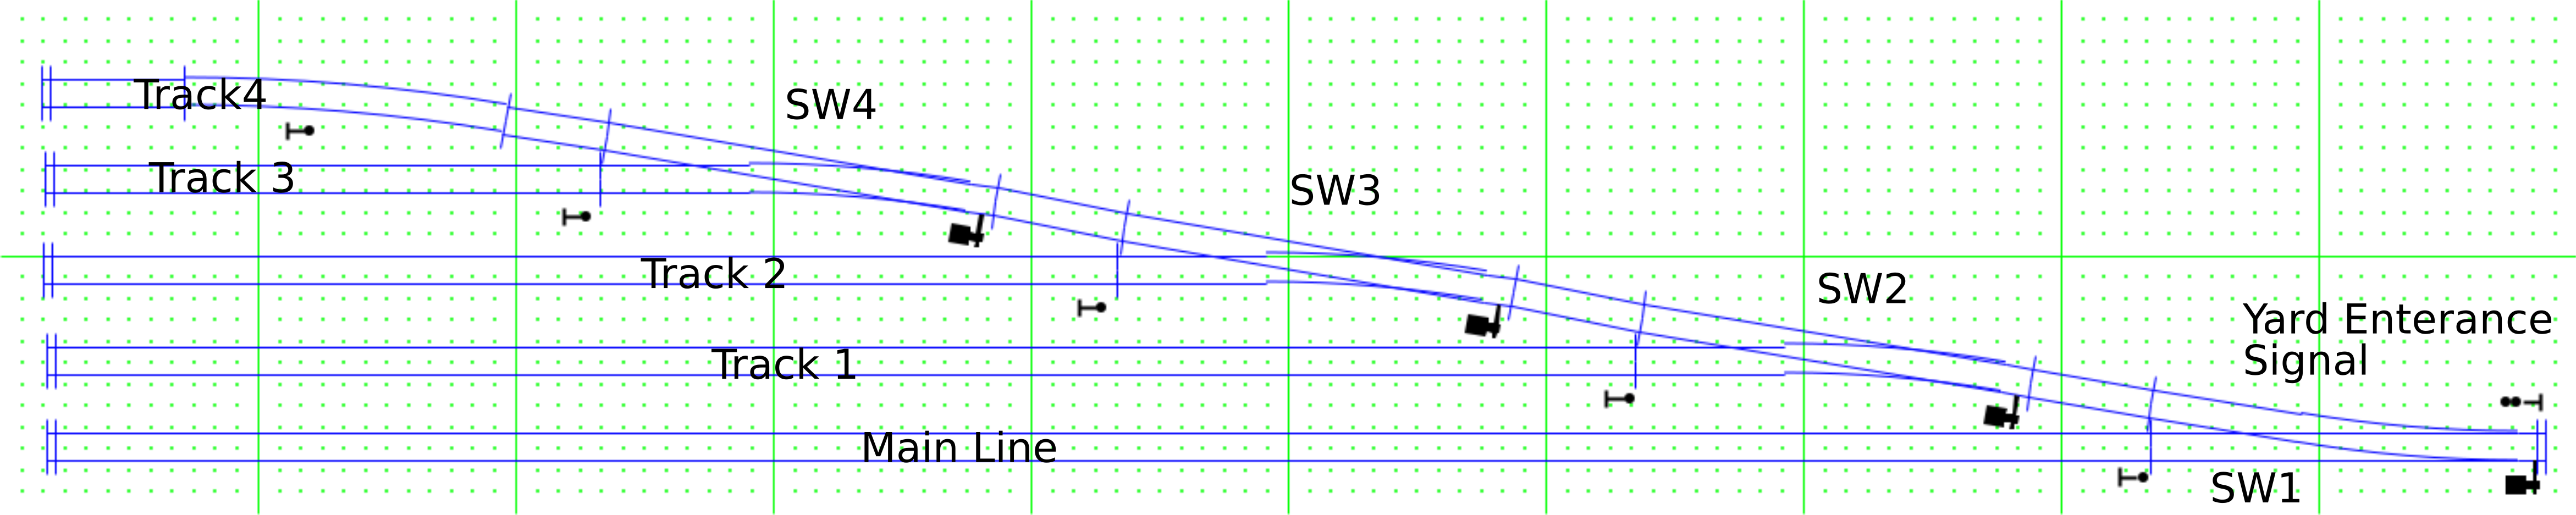
\includegraphics[width=4in]{ESP32S3-YardLadderAnnotated.png}
\caption{Yard Ladder}
\label{fig:YardLadder}
\end{centering}\end{figure}

The yard ladder shown in Figure~\ref{fig:YardLadder} has four yard tracks plus
the main line (at the bottom). There are four turnouts, which can be wired to
the four Stall Motors connections (see
Section~\ref{sec:StallMotorsconnections}). The main line can be broken up into
three ``blocks'': the track to the right of the bottom turnout, the bottom
turnout, and the track to the left of the bottom turnout. There is the 3 over
2 signal at the yard ladder entrance, the 3 color signal on the frog end of
the main (bottom) turnout. These two signals can use one bank of PWM signal
lamps. The other bank can be used for the four two-color dwarf (exit) signals
on the yard tracks. 
\begin{figure}[hbpt]\begin{centering}%
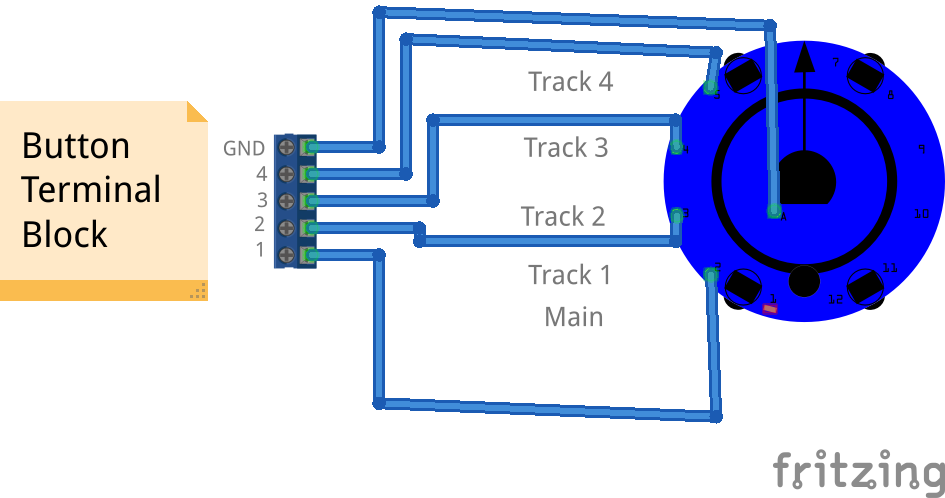
\includegraphics[width=4in]{ESP32S3-YardLadderRouteSelector_bb.png}
\caption{Yard Ladder Track Selector Switch}
\label{fig:YardLadderTrackSelectorSwitch}
\end{centering}\end{figure}
A simple way to control the yard would be with a 5 position single pole
rotatary switch. Positions 2-5 (''track 1'', ''track 2'', ''track 3'', and
''track 4'') would be wired to the four button inputs, with position 1
(''main'') left unconnected and the common to ground. These inputs would drive
logic cells to select five possible route: stay on main, divert to track 1,
track 2, track 3, or track 4 of the yard. See 
Figure~\ref{fig:YardLadderTrackSelectorSwitch}. A group of five logic cells 
could implement the routing:

\begin{verbatim}
if button1 then
  select track1: SW1 reversed, SW2 reversed
else if button2 then 
  select track2: SW1 reversed, SW2 normal, SW3 reversed
else if button3 then
  select track3: SW1 reversed, SW2 normal, SW3 normal,
                 SW4 reversed
else if button4 then
  select track4: SW1 reversed, SW2 normal, SW3 normal,
                 SW4 normal
else
  select main:   SW1 normal
\end{verbatim}


